\documentclass{standalone}
\usepackage{../preamble}
\def\xsep{0.35}
\def\eps{0.025}
\def\ysep{0.35}
\def\ysepB{0.25}
\def\y{2*\ysep+\ysepB+\eps}
\def\longtext{1.5}
\def\shorttext{0.5}
\def\points{0.075}
\def\colA{green!70!black!20}
\def\colB{yellow!40}
\def\linecol{black!50}
\begin{document}
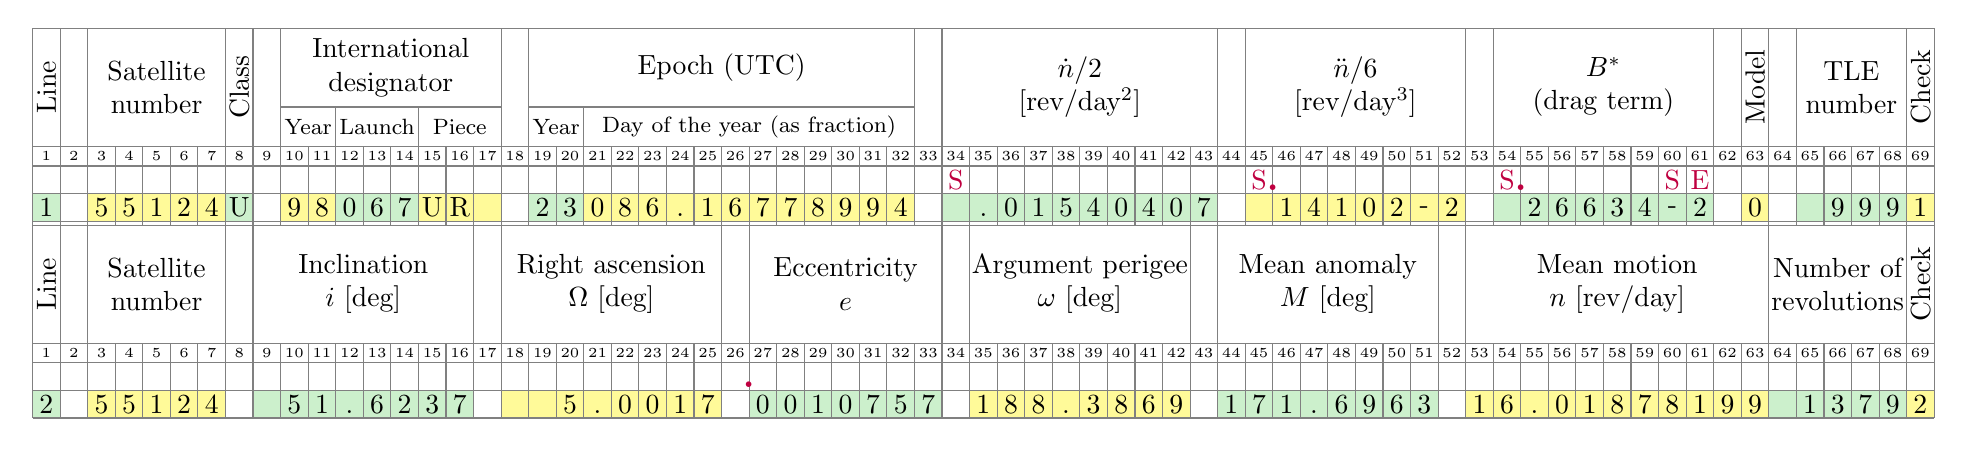
\begin{tikzpicture}
  % Color the boxes
  % Line 1
  \fill [\colA] ({0*\xsep},\eps) rectangle ({1*\xsep},\eps+\ysep);
  \fill [\colA] ({7*\xsep},\eps) rectangle ({8*\xsep},\eps+\ysep);
  \fill [\colA] ({11*\xsep},\eps) rectangle ({14*\xsep},\eps+\ysep);
  \fill [\colA] ({18*\xsep},\eps) rectangle ({20*\xsep},\eps+\ysep);
  \fill [\colA] ({33*\xsep},\eps) rectangle ({43*\xsep},\eps+\ysep);
  \fill [\colA] ({53*\xsep},\eps) rectangle ({61*\xsep},\eps+\ysep);
  \fill [\colA] ({64*\xsep},\eps) rectangle ({68*\xsep},\eps+\ysep);
  \fill [\colB] ({2*\xsep},\eps) rectangle ({7*\xsep},\eps+\ysep);
  \fill [\colB] ({9*\xsep},\eps) rectangle ({11*\xsep},\eps+\ysep);
  \fill [\colB] ({14*\xsep},\eps) rectangle ({17*\xsep},\eps+\ysep);
  \fill [\colB] ({20*\xsep},\eps) rectangle ({32*\xsep},\eps+\ysep);
  \fill [\colB] ({44*\xsep},\eps) rectangle ({52*\xsep},\eps+\ysep);
  \fill [\colB] ({62*\xsep},\eps) rectangle ({63*\xsep},\eps+\ysep);
  \fill [\colB] ({68*\xsep},\eps) rectangle ({69*\xsep},\eps+\ysep);

  % Line 2
  \fill [\colA] ({0*\xsep},-2*\ysep-\eps-\longtext-\ysepB) rectangle ({1*\xsep},-\eps-\longtext-\ysepB-\ysep);
  \fill [\colA] ({8*\xsep},-2*\ysep-\eps-\longtext-\ysepB) rectangle ({16*\xsep},-\eps-\longtext-\ysepB-\ysep);
  \fill [\colA] ({26*\xsep},-2*\ysep-\eps-\longtext-\ysepB) rectangle ({33*\xsep},-\eps-\longtext-\ysepB-\ysep);
  \fill [\colA] ({43*\xsep},-2*\ysep-\eps-\longtext-\ysepB) rectangle ({51*\xsep},-\eps-\longtext-\ysepB-\ysep);
  \fill [\colA] ({63*\xsep},-2*\ysep-\eps-\longtext-\ysepB) rectangle ({68*\xsep},-\eps-\longtext-\ysepB-\ysep);
  \fill [\colB] ({2*\xsep},-2*\ysep-\eps-\longtext-\ysepB) rectangle ({7*\xsep},-\eps-\longtext-\ysepB-\ysep);
  \fill [\colB] ({17*\xsep},-2*\ysep-\eps-\longtext-\ysepB) rectangle ({25*\xsep},-\eps-\longtext-\ysepB-\ysep);
  \fill [\colB] ({34*\xsep},-2*\ysep-\eps-\longtext-\ysepB) rectangle ({42*\xsep},-\eps-\longtext-\ysepB-\ysep);
  \fill [\colB] ({52*\xsep},-2*\ysep-\eps-\longtext-\ysepB) rectangle ({63*\xsep},-\eps-\longtext-\ysepB-\ysep);
  \fill [\colB] ({68*\xsep},-2*\ysep-\eps-\longtext-\ysepB) rectangle ({69*\xsep},-\eps-\longtext-\ysepB-\ysep);


  % Horizontal lines
  \draw[\linecol,thin] (0,-\eps-\longtext-\ysepB-\ysep-\ysep) -- ({69*\xsep},-\eps-\longtext-\ysepB-\ysep-\ysep);
  \draw[\linecol,thin] (0,-\eps-\longtext-\ysepB-\ysep) -- ({69*\xsep},-\eps-\longtext-\ysepB-\ysep);
  \draw[\linecol,thin] (0,-\eps-\longtext-\ysepB) -- ({69*\xsep},-\eps-\longtext-\ysepB);
  \draw[\linecol,thin] (0,-\eps-\longtext) -- ({69*\xsep},-\eps-\longtext);
  \draw[\linecol,thin] (0,-\eps) -- ({69*\xsep},-\eps);
  \draw[\linecol,thin] (0,\eps) -- ({69*\xsep},\eps);
  \draw[\linecol,thin] (0,\ysep+\eps) -- ({69*\xsep},\ysep+\eps);
  \draw[\linecol,thin] (0,2*\ysep+\eps) -- ({69*\xsep},2*\ysep+\eps);
  \draw[\linecol,thin] (0,\y) -- ({69*\xsep},\y);
  \draw[\linecol,thin] (0,\y+\longtext) -- ({69*\xsep},\y+\longtext);
  \draw[\linecol,thin] (9*\xsep,\y+\shorttext) -- ({17*\xsep},\y+\shorttext);
  \draw[\linecol,thin] (18*\xsep,\y+\shorttext) -- ({32*\xsep},\y+\shorttext);

  % vertical lines (secondary)
  \foreach \i in {11,14,20}{
      \draw[\linecol,thin] ({\i*\xsep},{\y}) -- ({\i*\xsep},{\y+\shorttext});
    }
  % long vertical lines (Line 1)
  \foreach \i in {0,1,2,7,8,9,17,18,32,33,43,44,52,53,61,62,63,64,68,69}{
      \draw[\linecol,thin] ({\i*\xsep},{\y}) -- ({\i*\xsep},{\y+\longtext});
    }
  % long vertical lines (Line 2)
  \foreach \i in {0,1,2,7,8,16,17,25,26,33,34,42,43,51,52,63,68,69}{
      \draw[\linecol,thin] ({\i*\xsep},{-\eps}) -- ({\i*\xsep},{-\eps-\longtext});
    }
  \foreach \i in {0,1,...,69}{
      \draw[\linecol,thin] ({\i*\xsep},{\y}) -- ({\i*\xsep},{-\eps});
      \draw[\linecol,thin] ({\i*\xsep},{-\eps-\longtext}) -- ({\i*\xsep},{-\eps-\longtext-\ysepB-\ysep-\ysep});-\ysep
    }
  \foreach \i in {1,2,...,69}{
      \node[font=\tiny] at ({(\i-1)*\xsep + \xsep/2},\ysepB/2+2*\ysep+\eps){\i};
      \node[font=\tiny] at ({(\i-1)*\xsep + \xsep/2},-\ysepB/2-\longtext-\eps){\i};
    }

  %
  %% Line 1 TLE: 1 55124U 98067UR  23086.16778994  .01540407  14102-2  26634-2 0  9991
  % \foreach \i/\j in{0/1,1/{ },2/5,3/5,4/1,5/2,6/4,7/U,8/{ },9/9,10/8,11/0,12/6,13/6,14/7,15/U,16/R,17/{ },18/2,19/3,20/0,21/8,22/6,23/.,24/1,25/6,26/7,27/7,28/8,29/9,30/9,31/4,32/{ },33/{ },34/{.},35/0,36/1,37/5,38/4,39/0,40/4,41/0,42/7,43/{ },44/{ },45/1,46/4,47/1,48/0,49/2,50/-,512  26634-2 0  9991}
  \foreach \i/\j in{0/1,1/{ },2/5,3/5,4/1,5/2,6/4,7/U,8/{ },9/9,10/8,11/0,12/6,13/7,14/U,15/R,16/{ },17/{ },18/2,19/3,20/0,21/8,22/6,23/{ },24/1,25/6,26/7,27/7,28/8,29/9,30/9,31/4,32/{ },33/{ },34/{ },35/0,36/1,37/5,38/4,39/0,40/4,41/0,42/7,43/{ },44/{ },45/1,46/4,47/1,48/0,49/2,50/-,51/2,52/{ },53/{ },54/2,55/6,56/6,57/3,58/4,59/-,60/2,61/{ },62/0,63/{ },64/{ },65/9,66/9,67/9,68/1}{
  \node[] at ({\i*\xsep + \xsep/2},\ysep/2+\eps){\j};
  }
  % dots in the bottom
  \foreach \i in {23,34}{
      \node[] at ({\i*\xsep + \xsep/2},\points+\eps){.};
    }
  % S and E 
  \node[purple] at ({33.5*\xsep},1.5*\ysep+\eps){S};
  \node[purple] at ({53.5*\xsep},1.5*\ysep+\eps){S};
  \node[purple,font=\Huge] at ({54*\xsep},\ysep+\eps+\points){.};
  \node[purple] at ({44.5*\xsep},1.5*\ysep+\eps){S};
  \node[purple,font=\Huge] at ({45*\xsep},\ysep+\eps+\points){.};
  \node[purple] at ({59.5*\xsep},1.5*\ysep+\eps){S};
  \node[purple] at ({60.5*\xsep},1.5*\ysep+\eps){E};

  % titles in the top
  \node[rotate = 90] at (\xsep/2,\y+\longtext/2){Line};
  \node[text width=1.5cm, align=center] at (4*\xsep+\xsep/2,\y+\longtext/2){Satellite number};
  \node[rotate = 90] at (7*\xsep+\xsep/2,\y+\longtext/2){Class};
  \node[text width=2cm, align=center] at (13*\xsep,{\y+\shorttext+(\longtext-\shorttext)/2}){International designator};
  \node[font=\footnotesize] at (10*\xsep,{\y+\shorttext/2}){Year};
  \node[font=\footnotesize] at (12.5*\xsep,{\y+\shorttext/2}){Launch};
  \node[font=\footnotesize] at (15.5*\xsep,{\y+\shorttext/2}){Piece};
  \node[] at (25*\xsep,{\y+\shorttext+(\longtext-\shorttext)/2}){Epoch (UTC)};
  \node[font=\footnotesize] at (19*\xsep,{\y+\shorttext/2}){Year};
  \node[font=\footnotesize] at (26*\xsep,{\y+\shorttext/2}){Day of the year (as fraction)};
  \node[text width=2cm, align=center] at (38*\xsep,\y+\longtext/2){$\dot{n}/2$ [rev/day$^2$]};
  \node[text width=2cm, align=center] at (48*\xsep,\y+\longtext/2){$\ddot{n}/6$ [rev/day$^3$]};
  \node[text width=2cm, align=center] at (57*\xsep,\y+\longtext/2){$B^*$\\(drag term)};
  \node[rotate=90] at (62.5*\xsep,\y+\longtext/2){Model};
  \node[text width=1.5cm, align=center] at (66*\xsep,\y+\longtext/2){TLE number};
  \node[rotate=90] at (68.5*\xsep,\y+\longtext/2){Check};

  % LINE 2: 2 55124  51.6237   5.0017 0010757 188.3869 171.6963 16.01878199 13792
  \foreach \i/\j in {0/2,1/{ },2/5,3/5,4/1,5/2,6/4,7/{ },8/{ },9/5,10/1,11/{ },12/6,13/2,14/3,15/7,16/{ },17/{ },18/{ },19/5,20/{ },21/0,22/0,23/1,24/7,25/{ },26/0,27/0,28/1,29/0,30/7,31/5,32/7,33/{ },34/1,35/8,36/8,37/{ },38/3,39/8,40/6,41/9,42/{ },43/1,44/7,45/1,46/{ },47/6,48/9,49/6,50/3,51/{ },52/1,53/6,54/{ },55/0,56/1,57/8,58/7,59/8,60/1,61/9,62/9,63/{ },64/1,65/3,66/7,67/9,68/2}{
  \node[] at ({\i*\xsep + \xsep/2},-1.5*\ysep-\eps-\longtext-\ysepB){\j};
  }
  % dots in the bottom
  \foreach \i in {11,20,37,46,54}{
      \node[] at ({\i*\xsep + \xsep/2},\points-2*\ysep-\eps-\longtext-\ysepB){.};
    }
  % S and E 
  \node[purple,font=\Huge] at ({26*\xsep},-\ysep-\ysepB-\eps-\longtext+\points){.};

  % titles in the top
  \node[rotate = 90] at (\xsep/2,-\eps-\longtext/2){Line};
  \node[text width=1.5cm, align=center] at (4*\xsep+\xsep/2,-\eps-\longtext/2){Satellite number};
  \node[text width=2cm, align=center] at (12*\xsep,-\eps-\longtext/2){Inclination\\$i$ [deg]};
  \node[text width=3.2cm, align=center] at (21*\xsep,-\eps-\longtext/2){Right ascension\\$\Omega$ [deg]};
  \node[text width=3.2cm, align=center] at (29.5*\xsep,-\eps-\longtext/2){Eccentricity\\$e$};
  \node[text width=3.2cm, align=center] at (38*\xsep,-\eps-\longtext/2){Argument perigee\\$\omega$ [deg]};
  \node[text width=3.2cm, align=center] at (47*\xsep,-\eps-\longtext/2){Mean anomaly\\$M$ [deg]};
  \node[text width=3.2cm, align=center] at (57.5*\xsep,-\eps-\longtext/2){Mean motion\\$n$ [rev/day]};
  \node[text width=1.7cm, align=center] at (65.5*\xsep,-\eps-\longtext/2){Number of revolutions};
  \node[rotate=90] at (68.5*\xsep,-\eps-\longtext/2){Check};
\end{tikzpicture}
\end{document}
